%!TEX root = kotov.tex
\section{Task 4: Сжатие путей и максимум на пути в дереве}
\begin{task}
    Дано дерево из $n$ вершин, с весами на рёбрах.
    Даны $m$ вертикальных путей (путь $a \leftarrow b$ вертикальный, если $b$ – предок $a$).
    Посчитайте на каждом вертикальном пути максимум весов рёбер. $n, m \leq 10^6$.
\end{task}

\begin{solution}
    Отсортируем все запросы по $b$ в порядке уменьшение глубины $b$ (за линию узнаем все глубины, т.е. $\O(n)$).
    Это будет стоить нам $\O(m\log m)$, для запросов с одинаковым $b$ оставляем их в обычном порядке, в котором пришли, это не важно.

    Теперь обрабатывает запросы в отсортированном порядке следующим образом: идем от вершины $a$ к вершине $b$ производя сжатие путей до $b$, причем, в процессе сжатия в качестве веса ребра указываем максимальный на пути от вершины до $b$, то есть каждая вершины $v$ на пути $a \rightarrow b$ будет подвешены к $b$, вес ребра --- наибольшее ребро на пути $v \rightarrow b$. В худшем, сложность будет $\O(n + m\log m)$.

    Почему это работает? Рассмотрим путь $a \rightarrow b \rightarrow c \rightarrow d$. Ясно, что самое тяжелое ребро на пути $a \rightarrow d$ --- это самое тяжелое из ребер на путях $a \rightarrow b$, $b \rightarrow c$ и $c \rightarrow d$, если сжать такие пути, то это просто вопрос о том, какой из ребер $a \rightarrow b$, $b \rightarrow c$ и $c \rightarrow d$ самое тяжелое. А так как у нас запросы только вертикальные, то мы не можем иметь ситуации, когда путь в каком-то предке уходит в других детей, т.е. ветки детей остаются нетронутыми, разве что вместе со своим предком при сжатии куда-то поднимаются, но пути в плане самого тяжелого ребра не портятся. Так же это вообще никак не отражается на остальной части дерева (имеется в виду, что после каждого запроса максимум что меняется только поддерево на $b$).

    \begin{figure}[H]
        \centering
        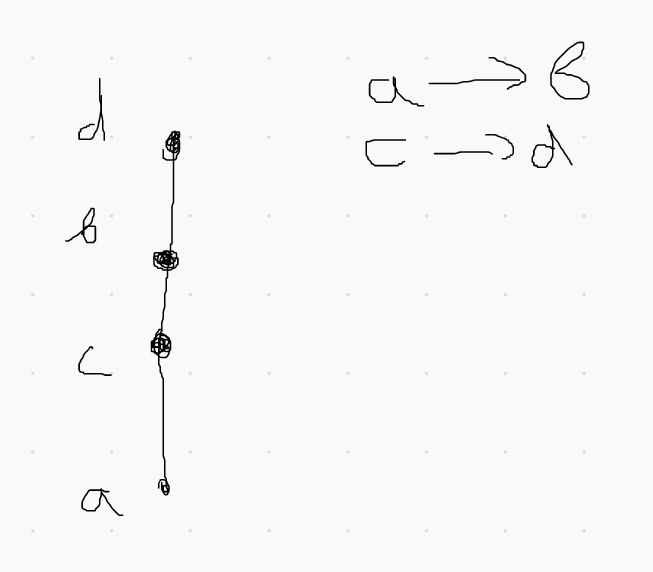
\includegraphics[width=0.5\textwidth]{pics/task4.png}
        \caption{Даже в такой ситуации, мы бы сначала сжали путь $a \rightarrow b$ и $c$ бы просто подвесилась бы к $b$, то есть мы ничего не потеряли в плане самого тяжелого ребра.}
    \end{figure}
\end{solution}